\documentclass[11pt,a4paper,parskip=half ]{scrartcl}
\usepackage[utf8]{inputenc}
\usepackage[ngerman]{babel}
\usepackage{amsmath}
\usepackage{amsfonts}
\usepackage{amssymb}
\usepackage{blkarray}
\usepackage{graphicx}
\usepackage{xcolor}
\usepackage{soul}

\usepackage{listings}
\lstset{
	numbers=left,
	showspaces=false,
	breaklines=true,
	tabsize=3,
	basicstyle=\ttfamily,
}

\author{Aaron Winziers - 1176638}
\title{Verteilte Informationssysteme WS 2019/20\\\LARGE{Übungsblatt 4}}

\begin{document}
	\maketitle
	
	\section*{Aufgabe 1}
	\paragraph{a)} Ein Semi-Join ist immer dann sinnvoll, wenn eine Beziehung zwischen den Reihen der beiden Tabellen vorhanden sein muss, aber die Informationen der einen TAbelle nicht benötigt werden. Wenn man eine Liste der Professoren die Vorlesungen halten haben will ohne wissen zu wollen was es für Veranstaltungen sind, könnte ein Semi-Join zwischen $professoren$ und $vorlesungen$ durchgeführt werden.
	
	\paragraph{b)} Die Matrikelnummer, Vornamen und Namen aller Studenten die im zweiten oder früheren Semester sind die eine oder mehrere Vorlesungen hören
	
	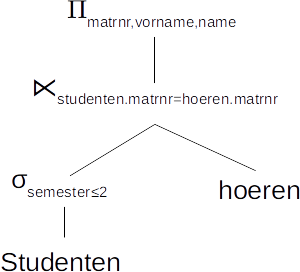
\includegraphics[scale=.7]{1b.png}
	
	
	\paragraph{c)} Die Matrikelnummer, Vornamen und Namen aller Studenten die im zweiten oder früheren Semester sind und die an einer Prüfung teilnehmen für die sie die Vorlesung nicht gehört haben.
	
	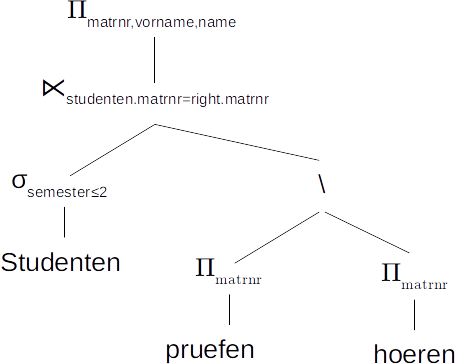
\includegraphics[scale=.7]{1c.png}
	
	\paragraph{d)} Die Matrikelnummer, Vornamen und Namen aller Studenten die im vierten oder früheren Semester sind, die eine Veranstaltung hören die 3 SWS oder mehr Aufwand haben und von dem Boss von dem Mitarbeiter mit Personalnummer 421337 gehalten werden.
	
	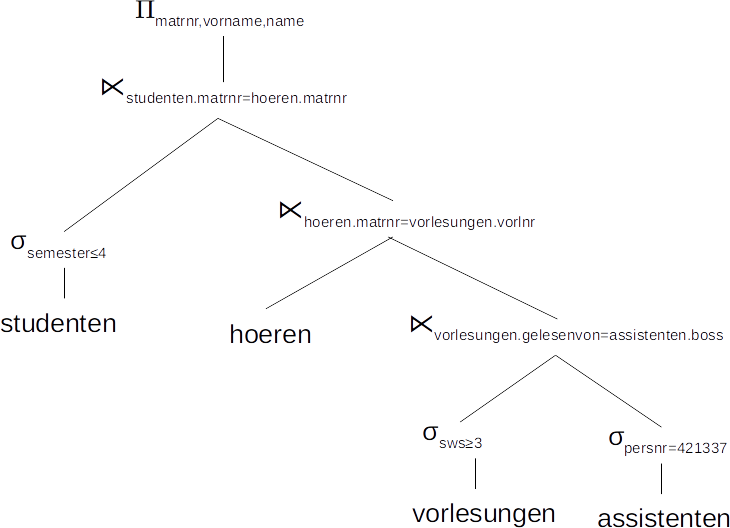
\includegraphics[scale=.6]{1d.png}
	
	
	In allen Fällen wurden die Selektionen und Projektionen so weit runter wie möglich in den Abfragebäumen gezogen um die Anzahl der Tupel die von den Joins verarbeitet werden müssen zu minimieren. Kartesische Produkte wurden durch Semi Joins so oft wie möglich ersetzt, erstens damit die Anzahl der resultierende Tupel stark reduziert wurde, und um die Größe der Tupel zu minimieren(nicht benötigte Daten zu sparen).
	
	Die unteren zwei Joins in Teilaufgabe d wurden mit Attribute ausgeführt die mit Hash Tabellen indexiert wurden was zu einer schnelleren Durchführung der Joins führen sollte. Da die Anzahl der Tupel in $hoeren$ sehr hoch ist sollte dies zu besserer Performance führen. Der letzte Join in der Aufgabe erfolg nicht mehr mittels Hash Tabellen, aber da die Anzahl der Tupel die in die rechte Seite des Joins kommen schon stark reduziert wurde sollte dies kein Problem darstellen.
	
	\newpage
	\section*{Aufgabe 2}
	\paragraph{a)} Hier wurden Selektionen wieder so weit runter in den Baum gezogen wie möglich. Hier wurde der Semi Join ausgeführt vor dem Natural Join, da die Partitionen $s_{1}$ und $h_{1}$ auf dem gleichen Knoten liegen, und somit weniger Daten zwischen den Knoten versendet werden mussten.
	
	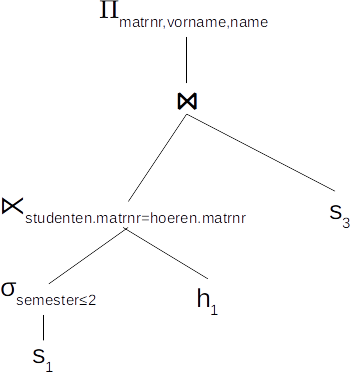
\includegraphics[scale=.6]{2a.png}
	
	\paragraph{b)} Da die Menge von Tupel die in $hoeren$ enthalten sind viel größer ist als die von $vorlesungen$, wurden die Partitionen von $vorlesungen$ redundant gejoined auf beiden Knoten die $h_{1}$ und $h_{2}$ enthalten. Dies sollte zu geringeren Kommunikationskosten führen, da nur eine reduzierte Menge an von $hoeren$ kommuniziert werden müsen.
	
	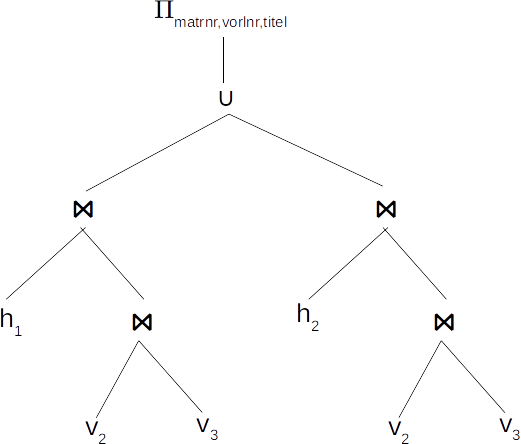
\includegraphics[scale=.6]{2b.png}
	
\end{document}
















